Zur Bestimmung der Rauschspektren wurden jeweils $16$ Datenspuren ohne angelegtes Signal mit einer Sampelrate von $f_s = \SI{100}{\kilo\hertz}$ aufgenommen.
Das Heißt die Nyquist-Frequenz, also die maximale auflösbare Frequenz, liegt bei $f_{Nq}=\SI{50}{\kilo\hertz}$.
Damit ist der interessante Teil des Spektrum abgedeckt.
Jenseits der $\SI{50}{\kilo\hertz}$ kommt dann der Effekt des Tiefpass zu tragen.
Für jede der Datenspuren wird die einseitige spektrale Leistungsdichte $J_{ss}(f_n)$ gemäß
\begin{equation}
\stackrel{\sim}{J}_{ss}(f_n) = 2 \frac{1}{N f_s}\left|\sum_i g(t_i)F(t_i)e^{-i\omega_n t_i}\right|^2
\end{equation}

\begin{minipage}[!c]{\textwidth}

\begin{minipage}[c]{\textwidth}
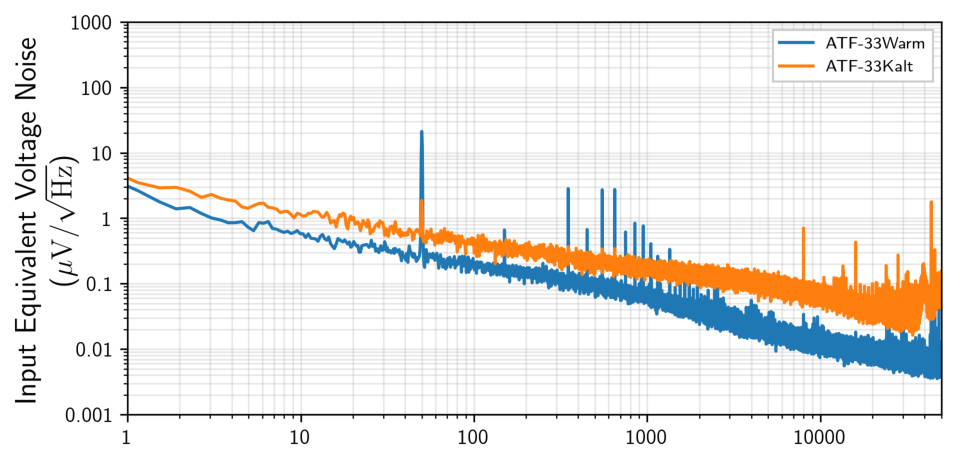
\includegraphics[width=\textwidth]{./fig/Rauschen/F33Warm.pdf}
\vspace{-0.45cm}
\captionof{subfigure}{Rauschen des HEMT ATF-33143}
\label{subfig:33}
\end{minipage}

\begin{minipage}[c]{\textwidth}
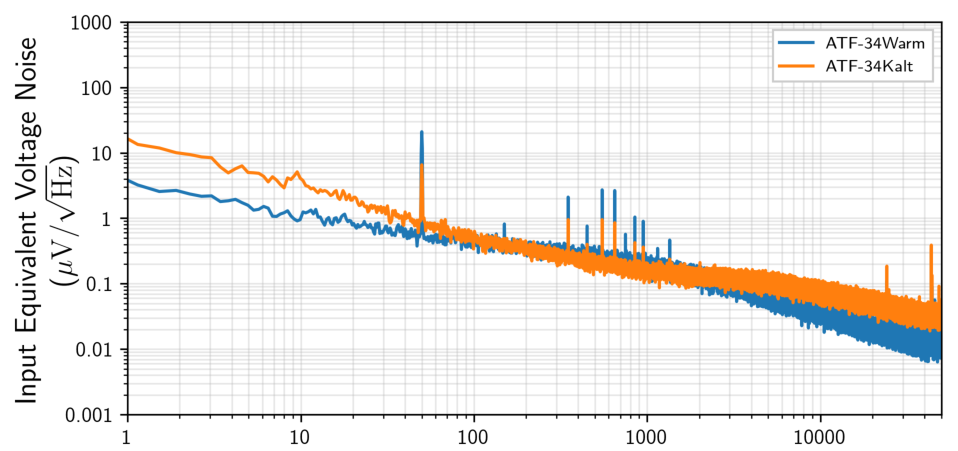
\includegraphics[width=\textwidth]{./fig/Rauschen/F34Warm.pdf}
\vspace{-0.45cm}
\captionof{subfigure}{Rauschen des HEMT ATF-34143}
\label{subfig:33}
\end{minipage}

\begin{minipage}[c]{\textwidth}
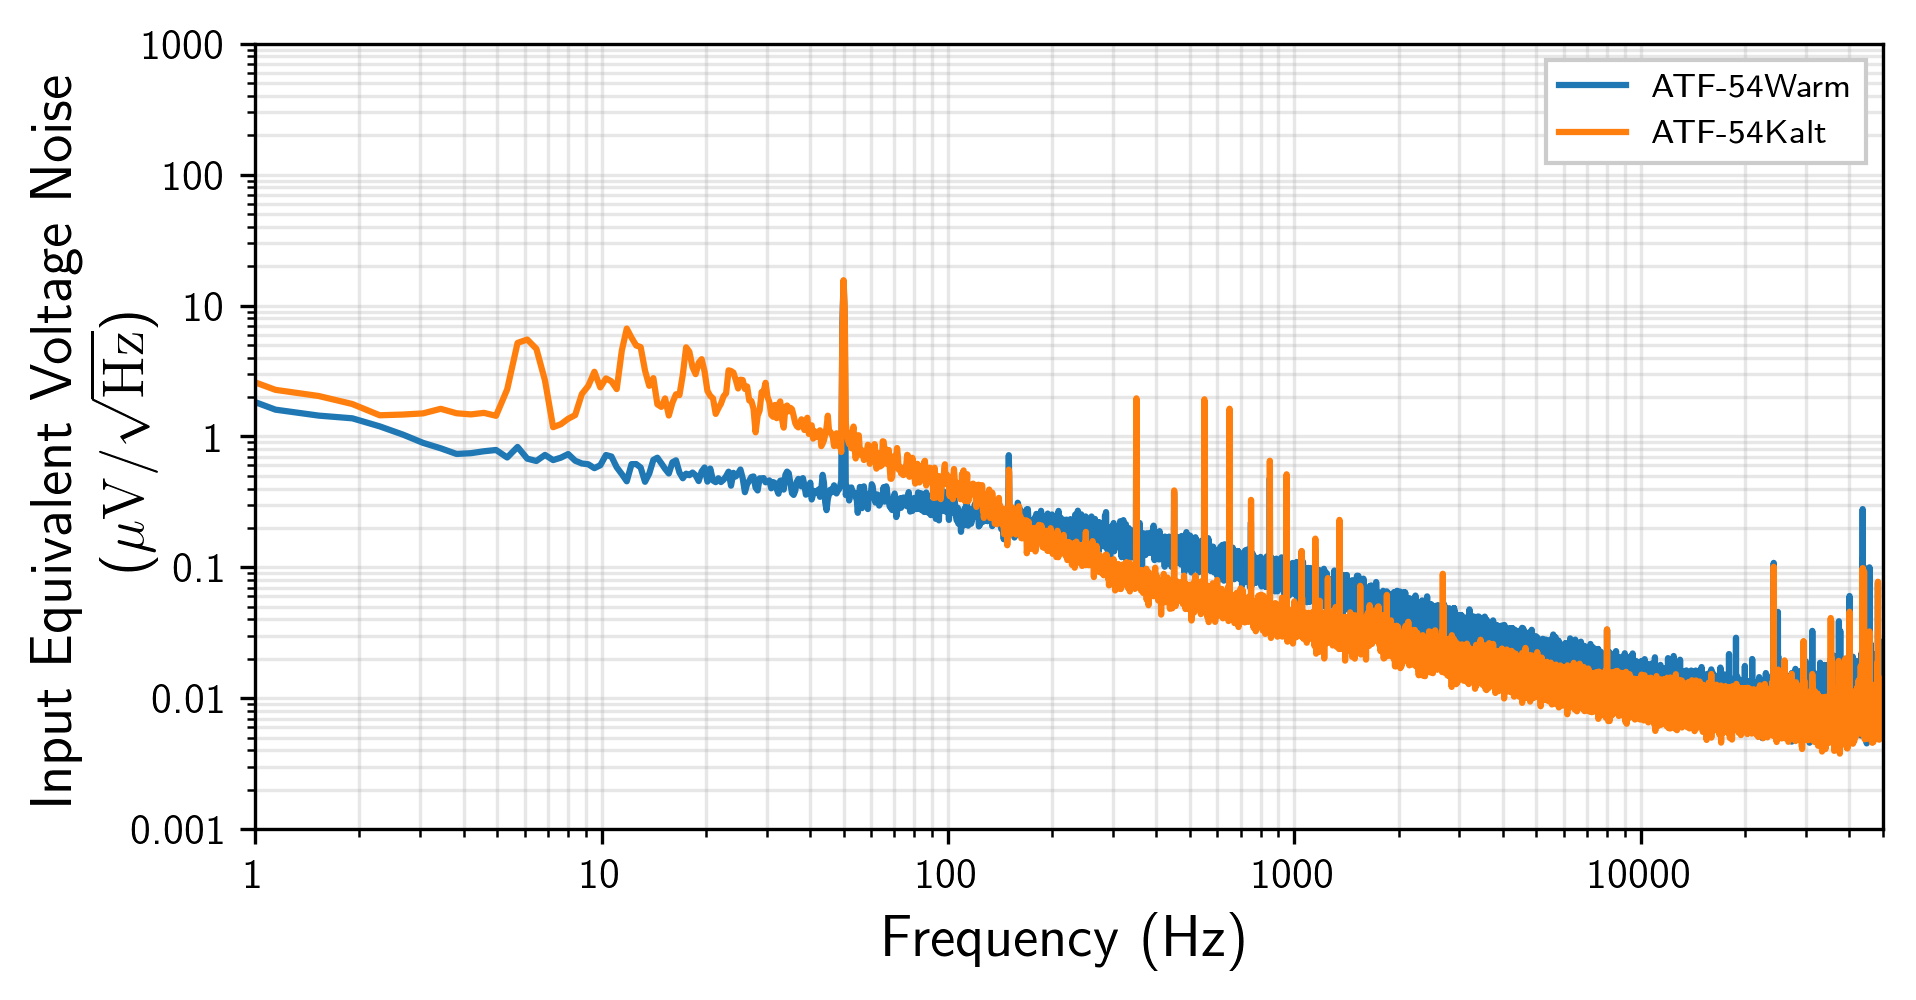
\includegraphics[width=\textwidth]{./fig/Rauschen/F54Warm.png}
\vspace{-0.45cm}
\captionof{subfigure}{Rauschen des HEMT ATF-54143}
\label{subfig:33}
\end{minipage}

\vspace{-0.4cm}
\captionof{figure}{Eingangsseitige Leistungsdichtespektren verschiedener HEMTs, bei geschlossenem Relais.
Bei Raumtemperatur (Warm) $\SI{291}{\kelvin}$ und bei flüssig Stickstoff Temperatur (Kalt) $\SI{77}{\kelvin}$.
Die gleiche Biasspannungen wie bei der Bestimmung der Verstärkung wurden verwendet.}
\label{fig:RauschenOpen}
\end{minipage}

mit der Fensterfunktion $F(t_i)$ bestimmt und über alle Spuren gemittelt.
Das auf diese weise erhaltene ausgangsseitige Leistungsspektrum wird durch das Quadrat der in Abschnitt \ref{sec:AuswertungAmp} erhaltenen Übertragungsfunktionen geteilt um das eingangs seitige Rauschen zu erhalten.

In Abbildung  ist $\sqrt{J_{ss}(f_n)}$ der verschiedenen HEMTs und Temperaturen dargestellt.
Alle Spektren weisen den erwarteten $\SI{50}{\hertz}$ Peak und seine harmonischen auf.
Mit der Verwendung von Batterien konnte dieser allerdings deutlich verringert werden.
Abgesehen davon treten im niederfrequenten Bereich sonst keine dominanten Peaks aus.
Erst im höherfrequenten Bereich jenseits der $\SI{10}{\kilo\hertz}$ treten vereinzelte Peaks auf welche vermutlich auf Umwelt Störeinflüsse zurückzuführen sind da sie nicht einheitlich bei allen Spektren auftreten.
Auffallend ist allerdings, dass für alle Spektren das Rauschen im niederfrequenten Bereich deutlich ansteigt bei flüssig Stickstoff Temperatur.
Eine mögliche Erklärung könnte sein, dass durch das sieden des Flüssigen Stockstoff Vibrationen entstehen welche in die Elektronik einkoppeln können.
Die gleichen Beobachtungen wurde auch in den Rauschspektren der EDELWEISS-III Ausleseelektronik von Axel Gullasch gemacht \cite{Gullasch2015}.
Da die Elektronik unmittelbar in den siedende Stickstoff eingetaucht wurde könnte dieser Effekt hier sogar noch größer sein.

Das beste Rauschspektrum ist in Abbildung \ref{fig:54RClosed} dargestellt und wurde wie erwartet bei offenem Relais erreicht, da das Rauschen durch die Biaswiderstände, Kabel und Spannungsquellen nicht mehr auftritt.
Im Vergleich mit dem Besten Rauschen der EDELWEISS-III Ausleselektronik \ref{fig:EDWIII} ist zu sehen, dass der HEMT basierte Verstärker ein deutlich geringeres Rauschen vor allem im niederfrequenten Bereich aufweist.
Hinzu kommt, dass der Auftretende $\SI{50}{\hertz}$ Peak und seine Harmonischen eine deutlich geringere Amplitude aufweisen.

\begin{figure}[!b]
\begin{center}
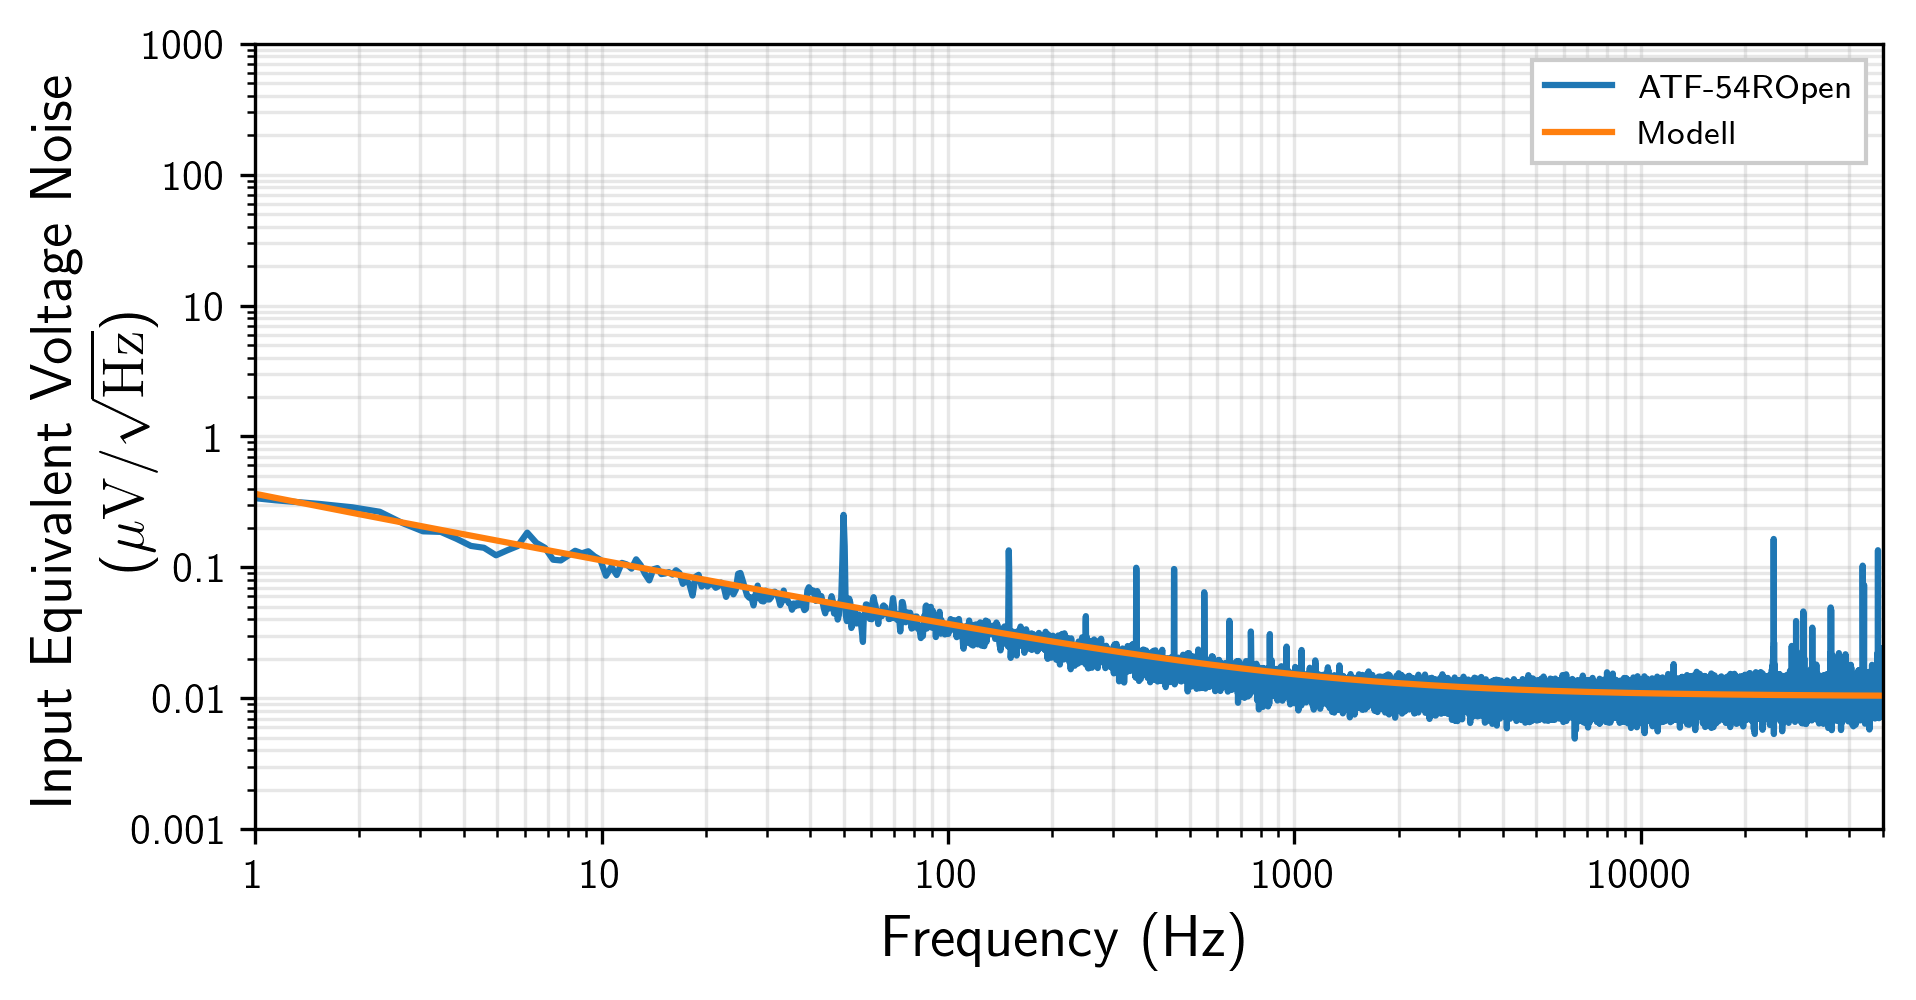
\includegraphics[width=\textwidth]{./fig/Rauschen/F54ROpen.png}
\vspace{-0.5cm}
\caption{Rauschen des HEMTs  ATF-54143 bei offenem Relais und einer Biasspannung von $\SI{0.371}{\volt}$.}
\label{fig:54ROpen}
\end{center}
\end{figure}

Das in Abschnitt \ref{sec:Rauschen} beschriebene Modell zur Beschreibung des Rauschen wurde an die gemessenen Daten Angepasst.
Da sich die gemessenen Daten sowohl aus dem Rauschen der Spannungsquelle $u_r$ und dem der Stromquelle $i_r$ zusammensetzen ist die Bestimmung des Rauschen der einzelnen quellen nicht möglich.
Für das gesamte Rauschen ergibt sich dann
\begin{equation}
u^2_{ges} = \frac{(\SI{8.3e-8}{})^2}{f^2} + \frac{(\SI{3.5e-7}{})^2}{f} + (\SI{1.0e-8}{})^2 \quad (\SI{}{\volt\squared\per\hertz}).
\end{equation}
Um das Rauschen der Quellen einzeln zu bestimmen muss zuerst der Eingang des Verstärkers geerdet werden dadurch verschwindet das Rauschen der Stromquelle und das der Spannungsquelle kann bestimmt werden.
Im Anschluss kann dann bei bekanntem rauschen der Spannungsquelle das der Stromquelle bestimmt werden.

Der Leckstrom wird aus dem Schortrauschen bestimmt.
Ein Vergleich des gemessenen $1/f^2$-Rauschen mit dem theoretisch erwarteten entsprechend Gl. \ref{eq:Rauschen} zeigt
\begin{equation}
\frac{a + 2eI_{Leck}}{4\pi^2C^2_{ges}} = (\SI{8.3e-8}{})^2.
\end{equation}
Mit der Annahme, dass der Parameter $a=0$ ist ergibt sich für den Leckstrom eine obere Abschätzung von
\begin{equation}
I_{Leck} = \SI{1.4}{\femto\ampere}.
\end{equation}

\begin{figure}[!b]
\begin{center}
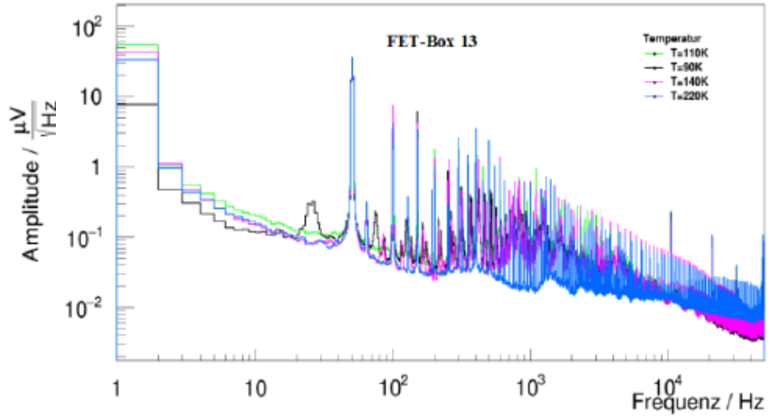
\includegraphics[width=\textwidth]{./fig/Rauschen/GullaschRauschen.pdf}
\vspace{-0.5cm}
\caption{Beste Leistungsdichtespektren der EDELWEISS-III Ausleseelektronik von Axel Gullasch \cite{Gullasch2015}.}
\label{fig:EDW}
\end{center}
\end{figure}